\chapter{Impact of APV25 saturation on displaced tracking}
\label{k0}
A portion of the data collected by the CMS detector in 2016 is affected by the APV saturation effect described in Ref.~\cite{hip_study}. The APV25 saturation effect is a byproduct of the production of heavily ionising particles (HIPs) in inelastic interactions between hadrons and the nuclei of silicon sensors. The energy deposits of HIPs can be up to 1000 times greater than those of typical particles produced in LHC collisions. These large energy deposits can saturate the analog readout of the APV25 chips~\cite{apv25} that are used to read out the CMS silicon strip tracker, which is described in Section~\ref{tracker}. Due to a feature of the APV25 powering scheme that normally helps stabilize the pulse-height baseline, a single saturated channel can inadvertently suppress the outputs of the 127 other APV25 channels for hundreds of nanoseconds.

Only around one in every 1000 incident hadrons will result in saturating HIP events, so the effect is only significant at high instantaneous luminosities. In 2016, the instantaneous luminosity increased to greater than the original LHC design goal, and the effect began influencing detector performance. Starting in run 278802, the tracker front-end electronics were reconfigured to substantially reduce their sensitivity to the APV25 saturation effect.

The deadtime associated with the a saturating HIP event can cause some tracker hits to be lost. This effect can lead to reduced tracking efficiency, and it is reasonable to suspect that the lose of efficiency may be more significant for displaced particles that may have fewer tracker hits to begin with. To investigate the impact on displaced tracking, one of our collaborators, Ian Tomalin, performed a study with $\Kzero\to\pi^+\pi^-$ decays. From this study, we conclude that only data taken after the APV25 saturation effect was mitigated should be used in the Displaced Leptons analysis. We therefore use only eras G and H in 2016 and all available data from 2017 and 2018.

Using data collected in 2016, 2017, and 2018 with the \texttt{HLT\_ZeroBias} trigger, the reconstructed \Kzero candidate decay lengths are compared among several different runs that correspond to a wide range of instantaneous luminosities and data-taking periods. The \Kzero candidates used come from the \texttt{generalV0Candidates:Kshort} collection. Each candidate must have a pair of oppositely charged tracks consistent with the \Kzero mass and coming from a common vertex that is at least \SI{2}{\cm} from the beam line. The tracks are required to have at least one pixel hit and $|\eta|<2$. In 2016 (2017-18), the tracks are required to have $\pt>\SI{0.7}{\GeV}\ (\SI{1.5}{\GeV})$.

Figure~\ref{k0_tracking_eff} shows the reconstructed transverse decay length of the \Kzero candidates for data from all three years. Each distribution is normalized to the integrated luminosity of the run from which it is taken. In the 2016 plot, the solid (dashed) lines correspond to runs taken before (after) the APV25 saturation effect was mitigated. In the pre-mitigation runs, the \Kzero transverse decay length distribution falls rapidly with increasing instantaneous luminosity, but the dependence on instantaneous luminosity is significantly reduced in the post-mitigation runs and in all 2017 and 2018 runs. The narrower transverse decay length at higher luminosity in the 2016 pre-mitigation runs is interpreted as an instantaneous-luminosity-dependent decrease in tracking efficiency.

\begin{figure}
\centering
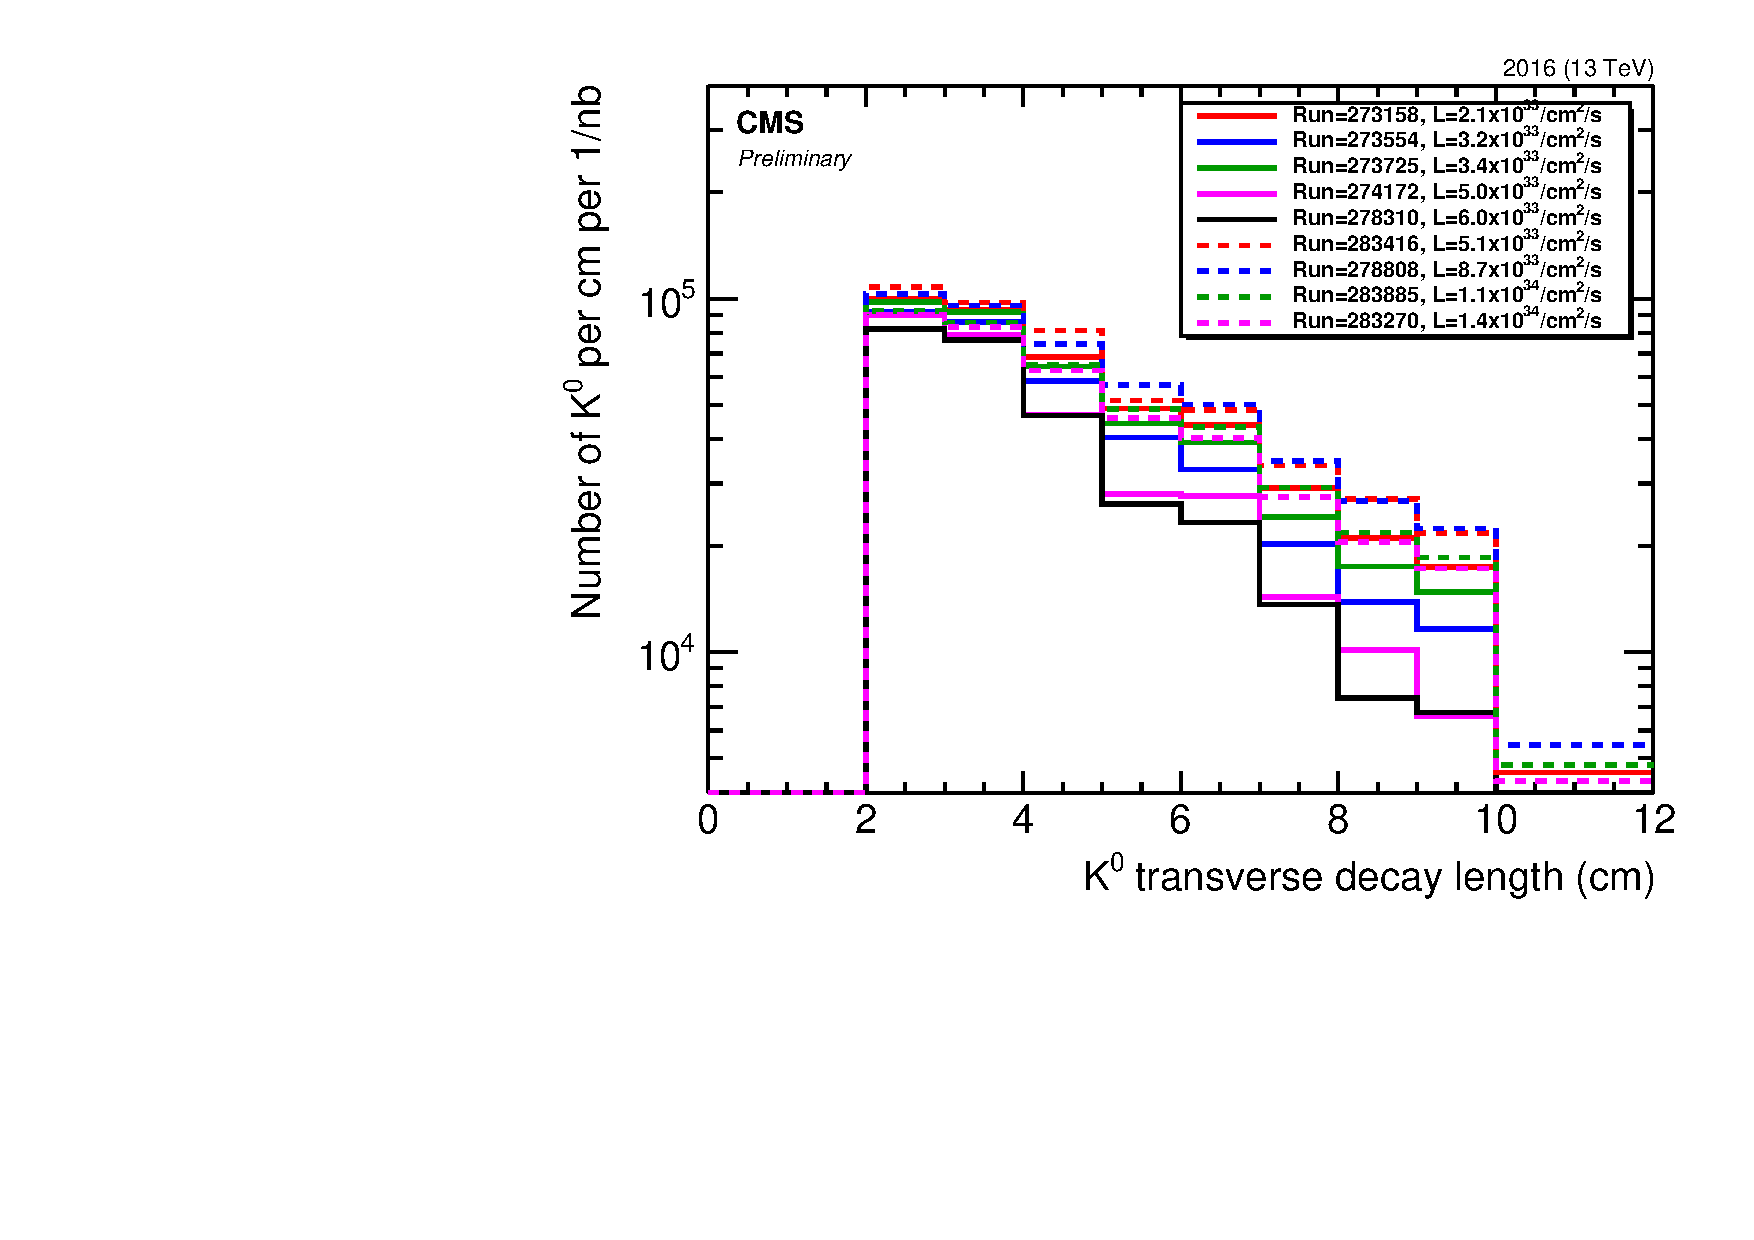
\includegraphics[width=0.45\textwidth]{figures/tracking_eff/2016/k0.pdf}
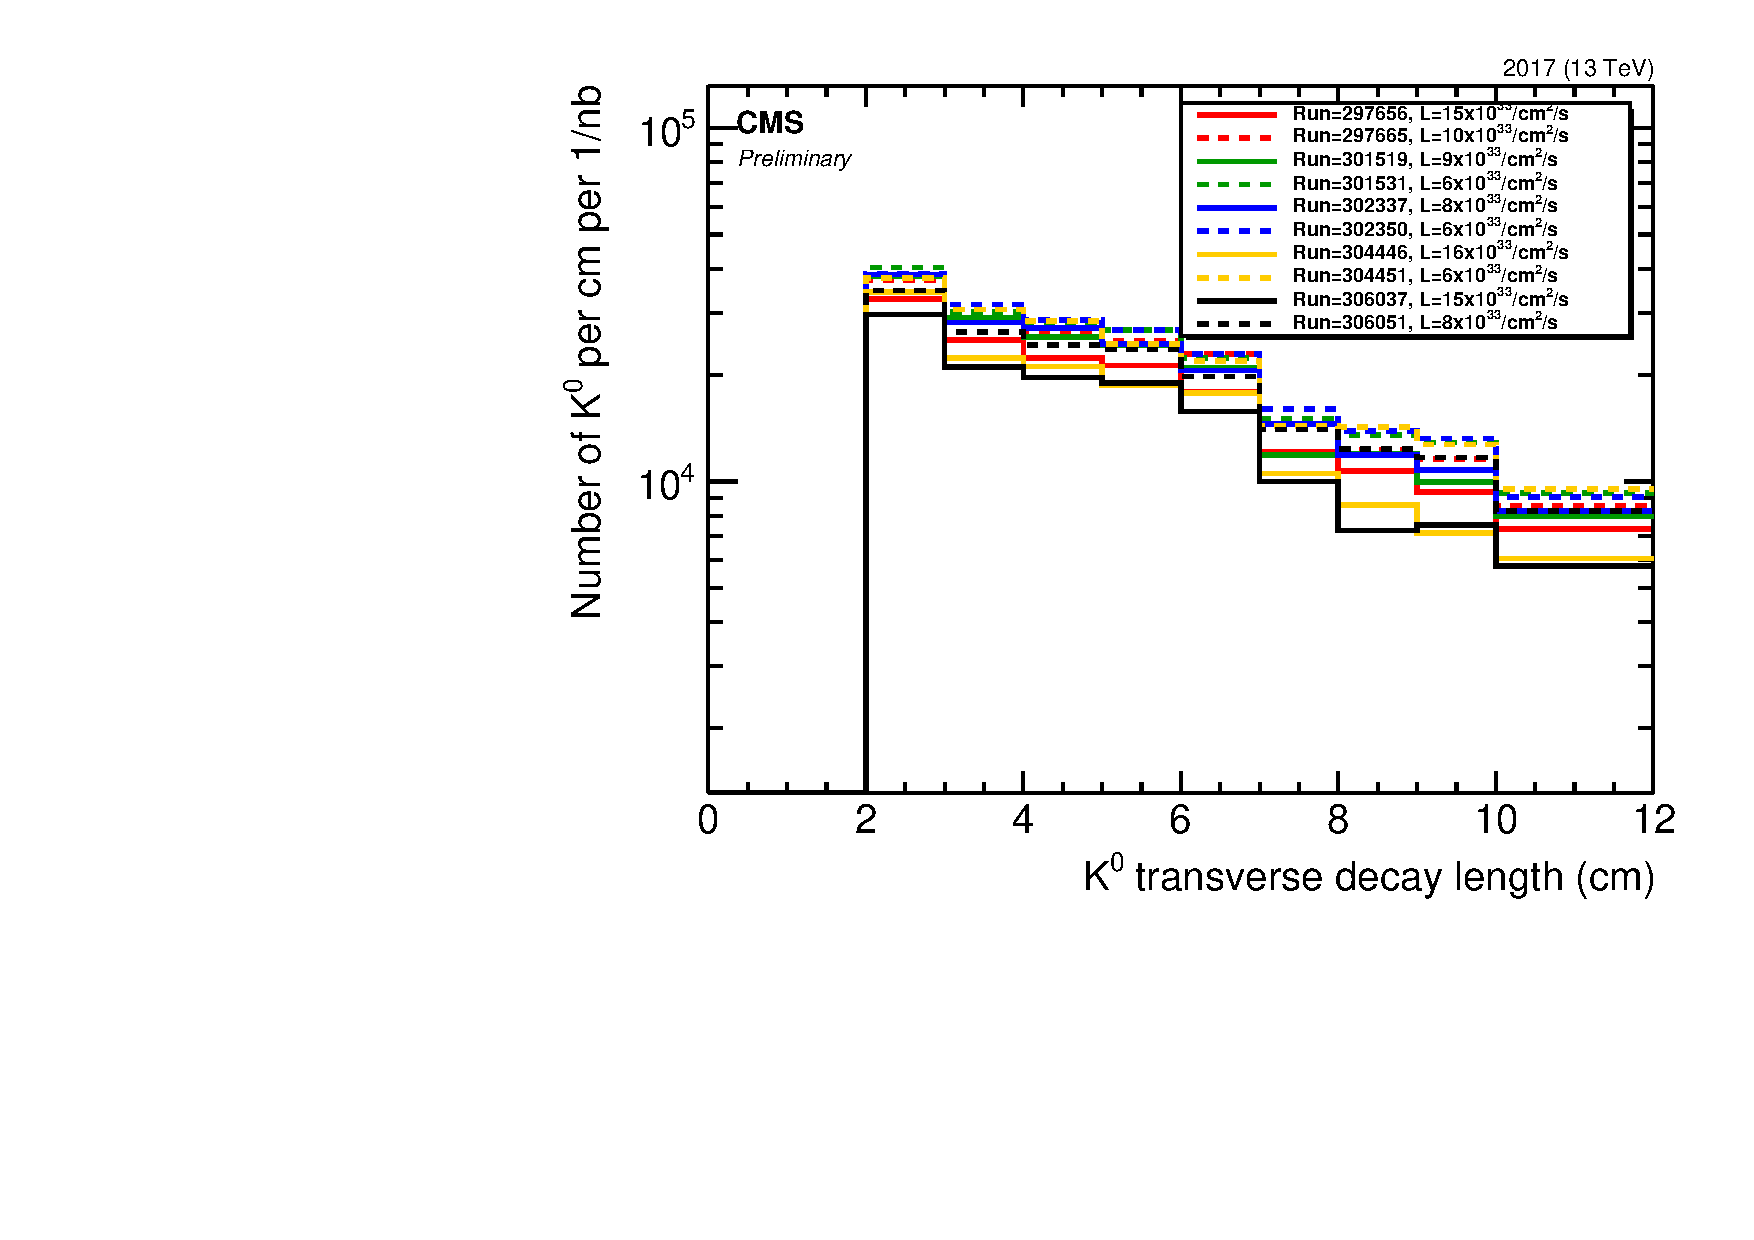
\includegraphics[width=0.45\textwidth]{figures/tracking_eff/2017/k0.pdf}
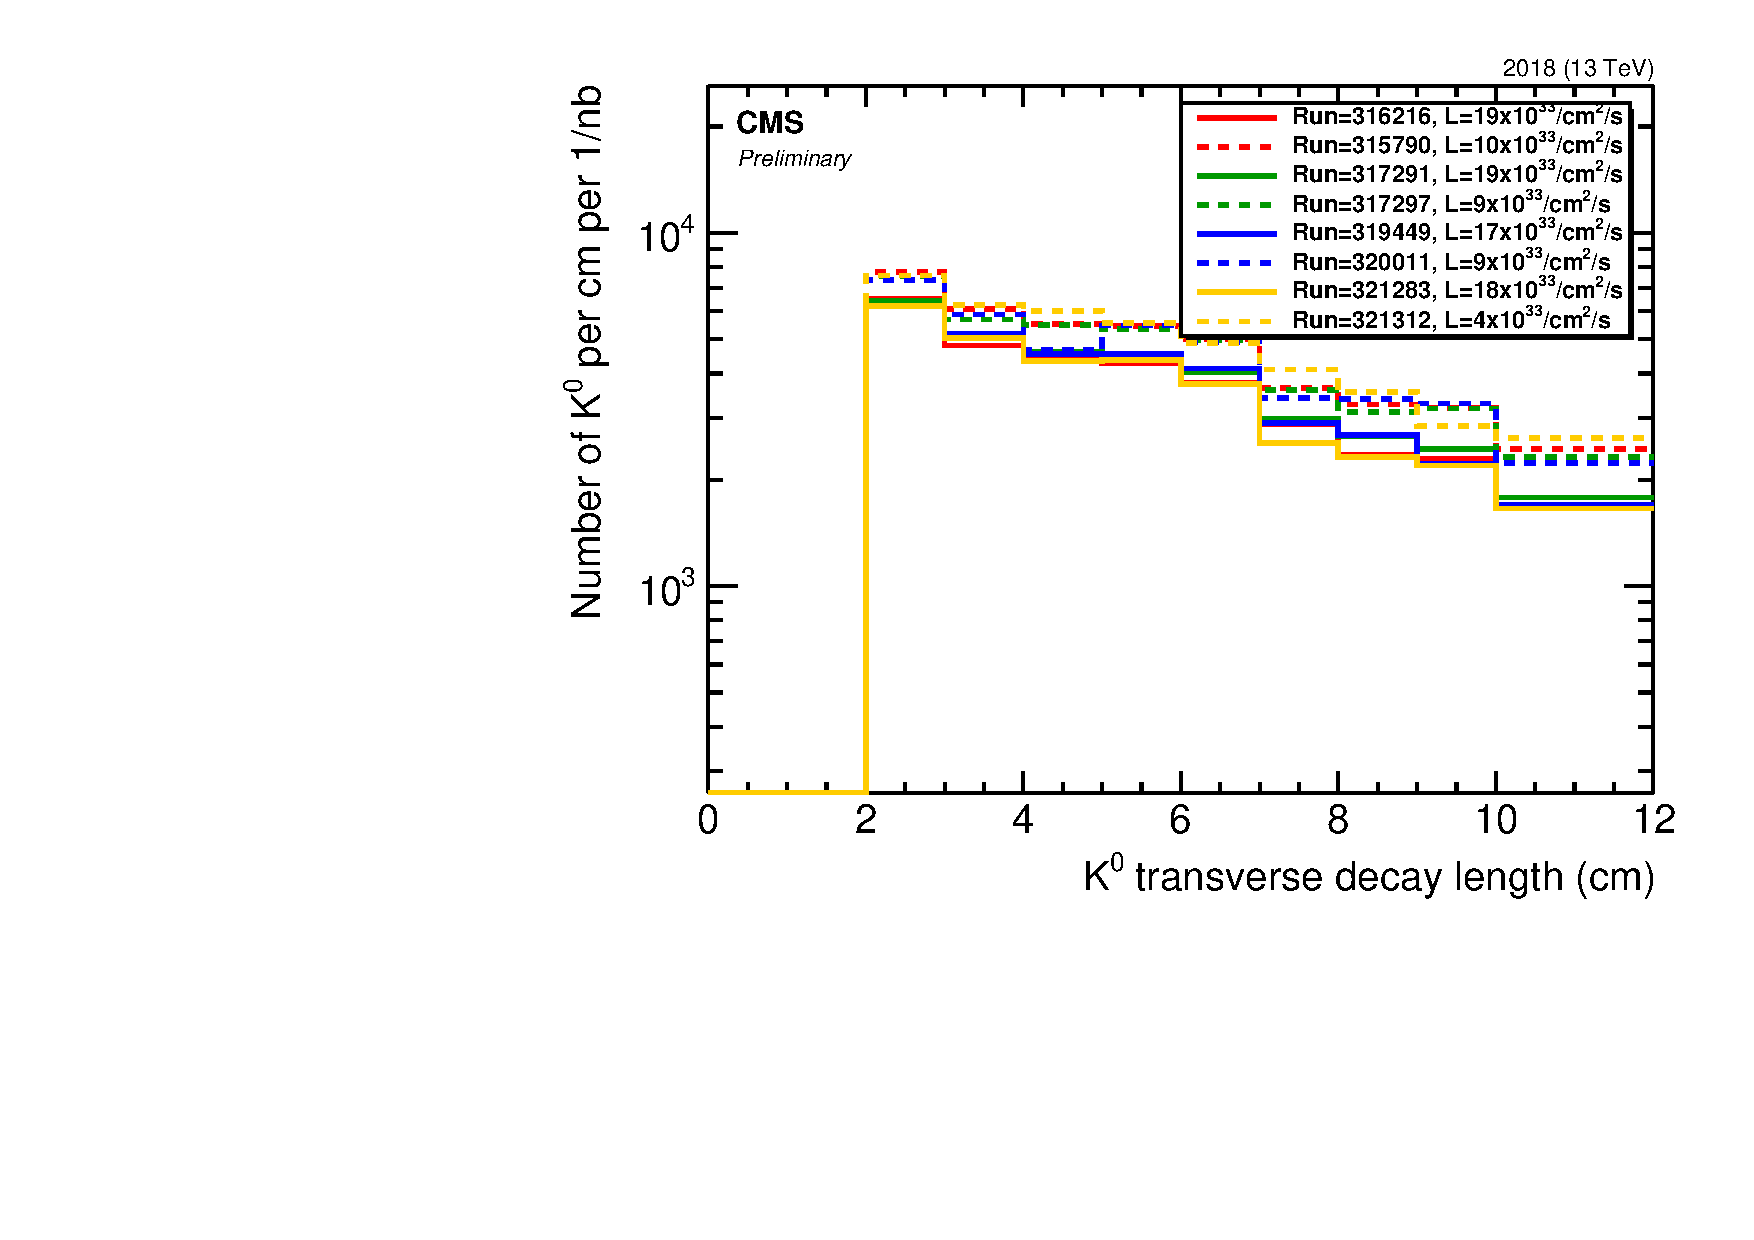
\includegraphics[width=0.45\textwidth]{figures/tracking_eff/2018/k0.pdf}
\caption{Transverse decay length distribution of reconstructed $\Kzero\to\pi^+\pi^-$ candidates for various runs in 2016 (top left), 2017 (top right) and 2018 (bottom). The peak instantaneous luminosity of each run is indicated in the legend, and each distribution is normalized to the integrated luminosity of the run. In the 2016 plot, runs taken before (after) the APV25 saturation effect was mitigated are shown by solid (dashed) lines. In the 2017 plot, the run with lowest (highest) instantaneous luminosity examined in each data-taking era is plotted with a dashed (solid) line. Towards the end of 2017 (orange and black lines) the LHC ran with approximately 20\% fewer proton bunches, meaning that the instantaneous luminosity per bunch crossing was higher than one might naively expect from the instantaneous luminosities shown in the legend.}
\label{k0_tracking_eff}
\end{figure}

Given the size of this effect, we decide not to use 2016 data taken before run 278802 in the Displaced Leptons search. The instantaneous-luminosity-dependent displaced tracking efficiency would be difficult to quantify, which would lead to large systematic uncertainties. Furthermore, the signal yield would be suppressed by the lower displaced tracking efficiency. Finally, studies of displaced tracking efficiency with cosmic ray data are insensitive to the APV25 saturation effect because the instantaneous luminosity during dedicated cosmic runs is zero.

A small dependence on instantaneous luminosity is also apparent in the 2017 and 2018 distributions shown in Fig.~\ref{k0_tracking_eff}. The runs with the lowest (highest) instantaneous luminosity examined in each data taking period are shown with dashed (solid) lines. This may be due to a residual APV saturation effect or possibly another luminosity-related tracker inefficiency. We do not find it necessary to take any special measures to account for this small effect in 2017 and 2018.

